\section{Parallelization}
\label{sec:dmsc_parallelization}
The parallelization complicates parts of the implementation steps described in section \ref{sec:dsmc_implementation_timestep}. For example, the file containing the geometry information is split into several files, one per processor. Each processor will then only know about a subset of the whole system geometry. To simplify this reading, we will only explain the basic philosophy of how the code is parallelized.

Each collision cell is completely independent of the other cells. We can then divide the spatial domain into sub domains, each fully controlled by one processor. Each processor is responsible for executing the timestep for every particle in the corresponding volume. The processors will usually contain many collision cells as illustrated in figure \ref{fig:dsmc_parallelization_1}. We will use the terms \textit{processor}, \textit{node} and \textit{CPU} interchangeably.
\begin{figure}[htb]
\begin{center}
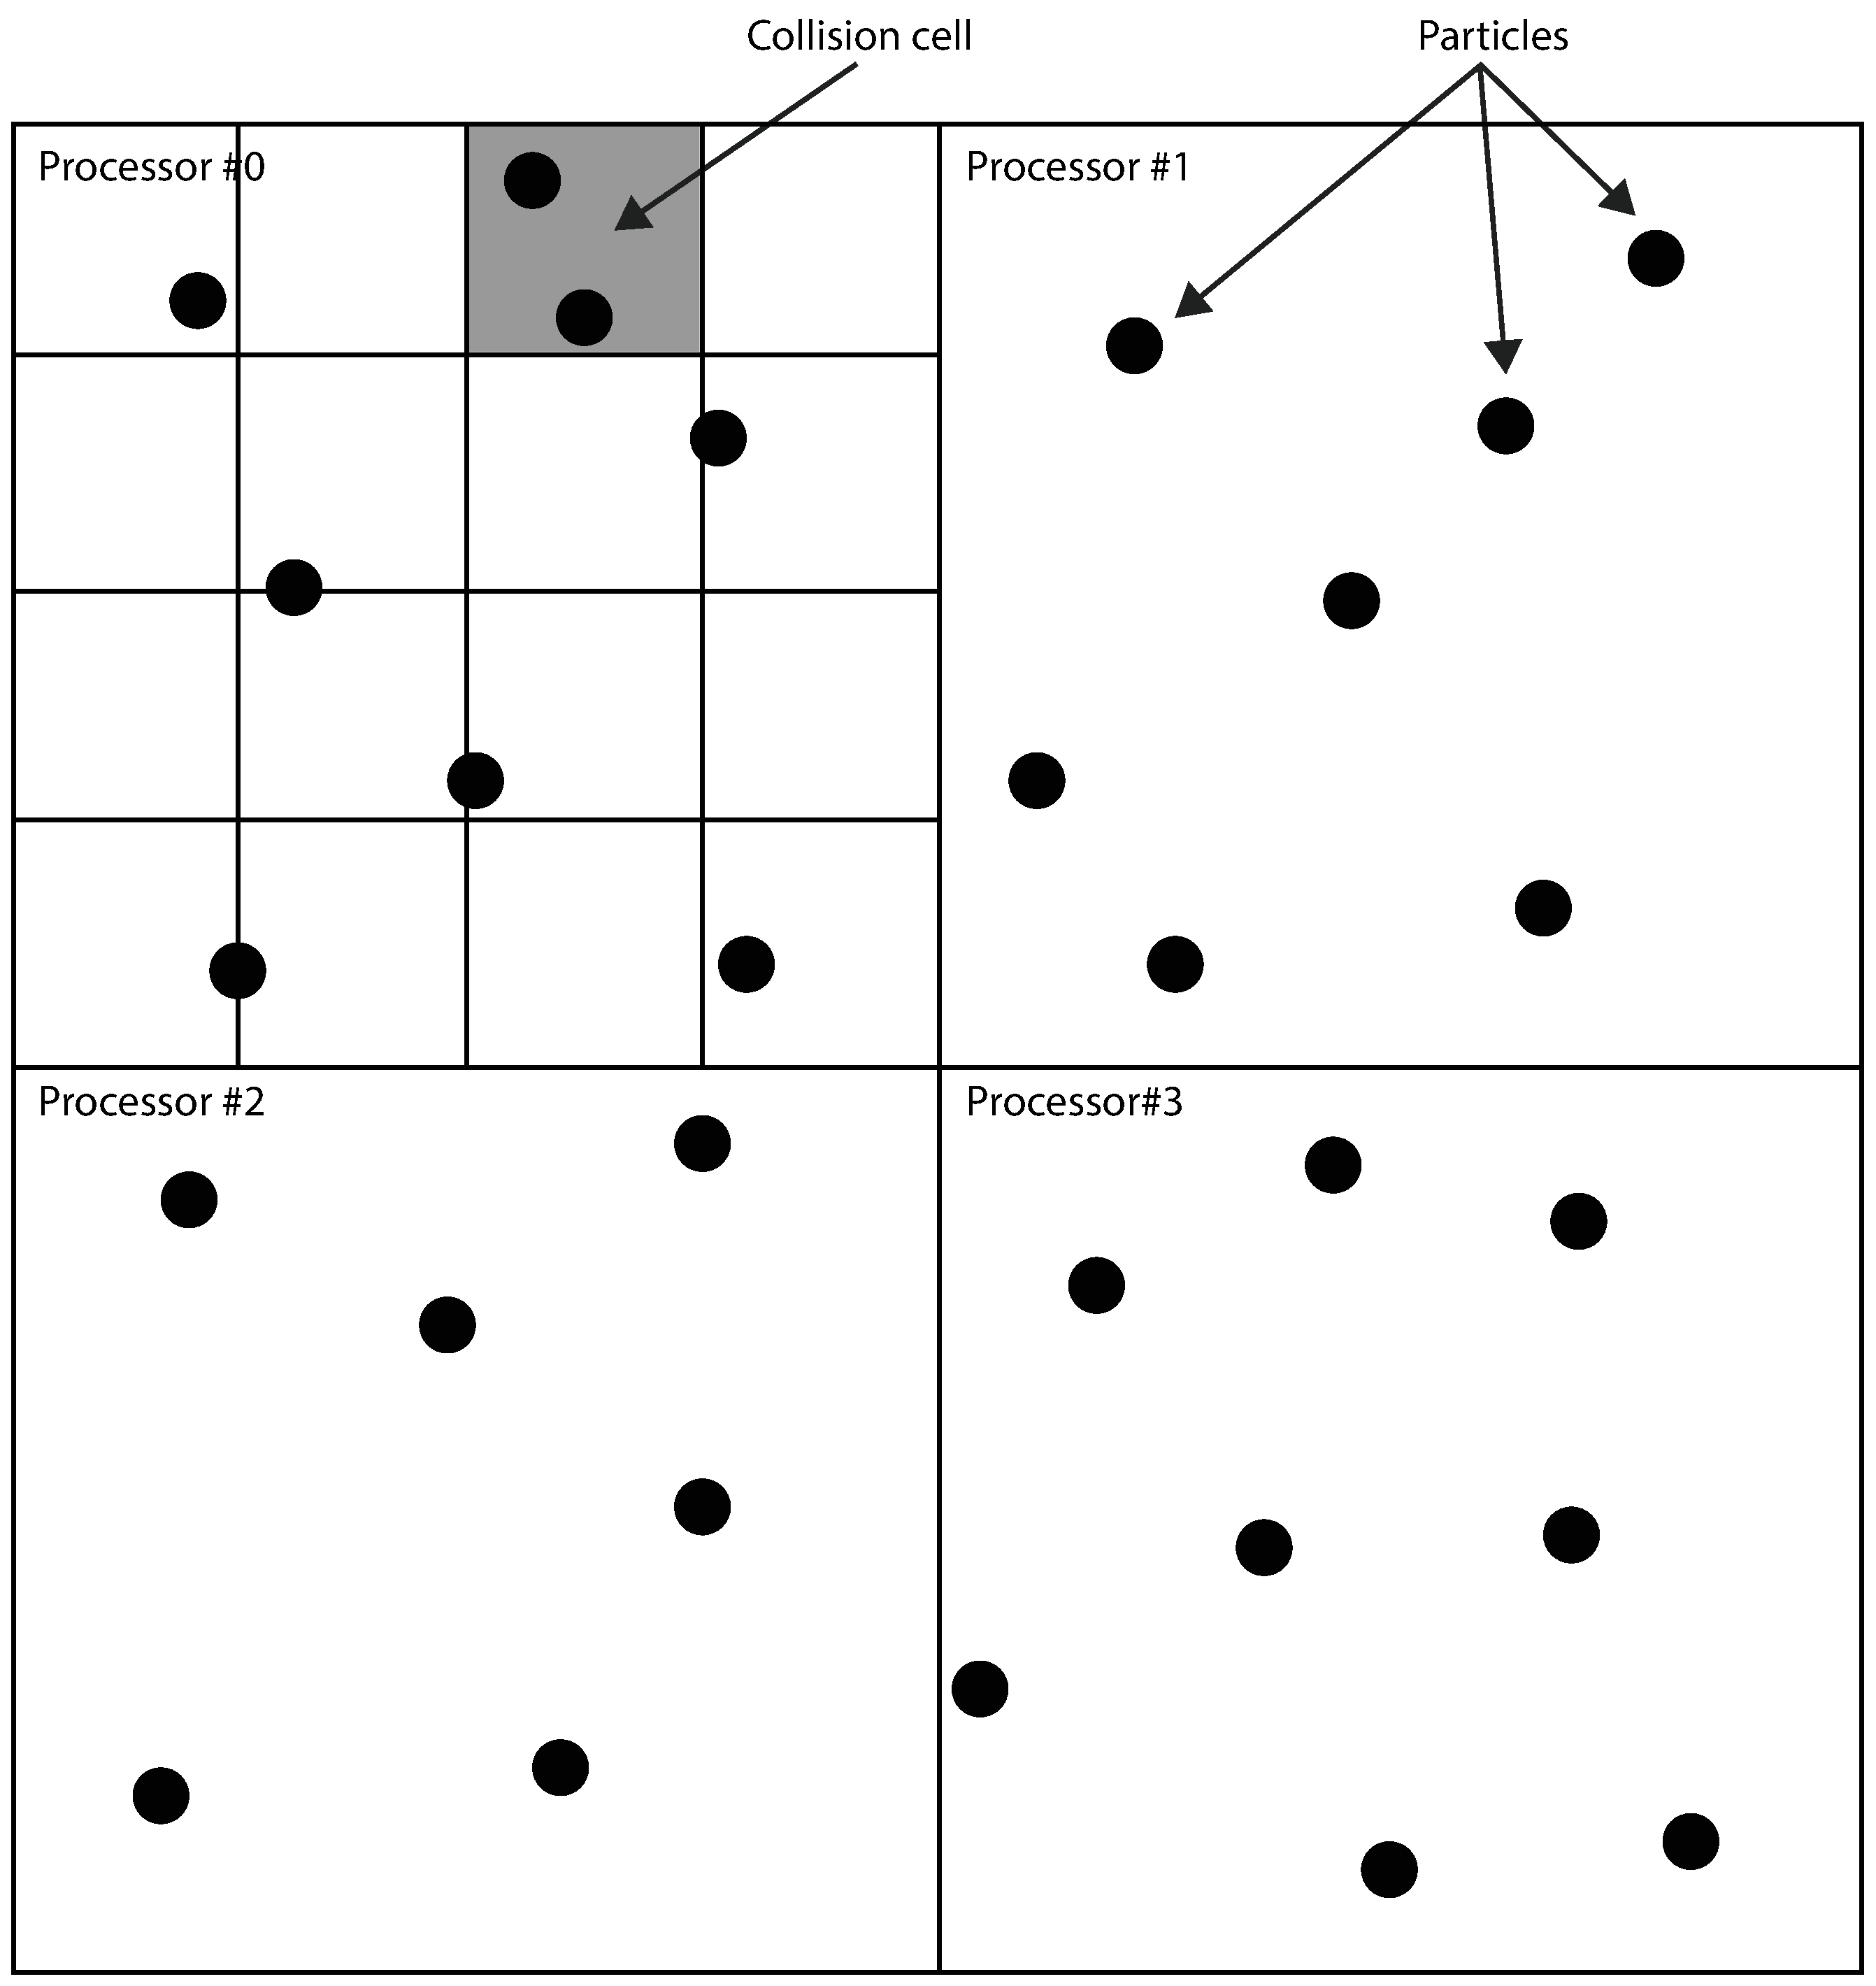
\includegraphics[width=0.7\textwidth, trim=0cm 0cm 0cm 0cm, clip]{DSMC/figures/parallelization.eps}
\end{center}
\caption{Illustration of how the spatial domain can be divided into four sub domains, each controlled by a processor. Each processor contains many particles that are placed in several collision cells (marked grey).}
\label{fig:dsmc_parallelization_1}
\end{figure}
Given that the processors have knowledge about the particles living in its volume, the only thing we have to take care of is when particles move from one processor to another. We have used (MPI) for the communication between processors, and assume that the reader is familiar with how MPI works. 
\subsection{Topological structure}
The processors are divided into a three dimensional grid with $(P_x, P_y, P_z)$ being the number of CPU's in each dimension, yielding a total of $P = P_xP_yP_z$ processors. We can then use the grid coordinates $(p_x, p_y, p_z)$ to uniquely label the processors as shown in figure \ref{fig:dsmc_parallelization_2}.
\begin{figure}[htpb]
\begin{center}
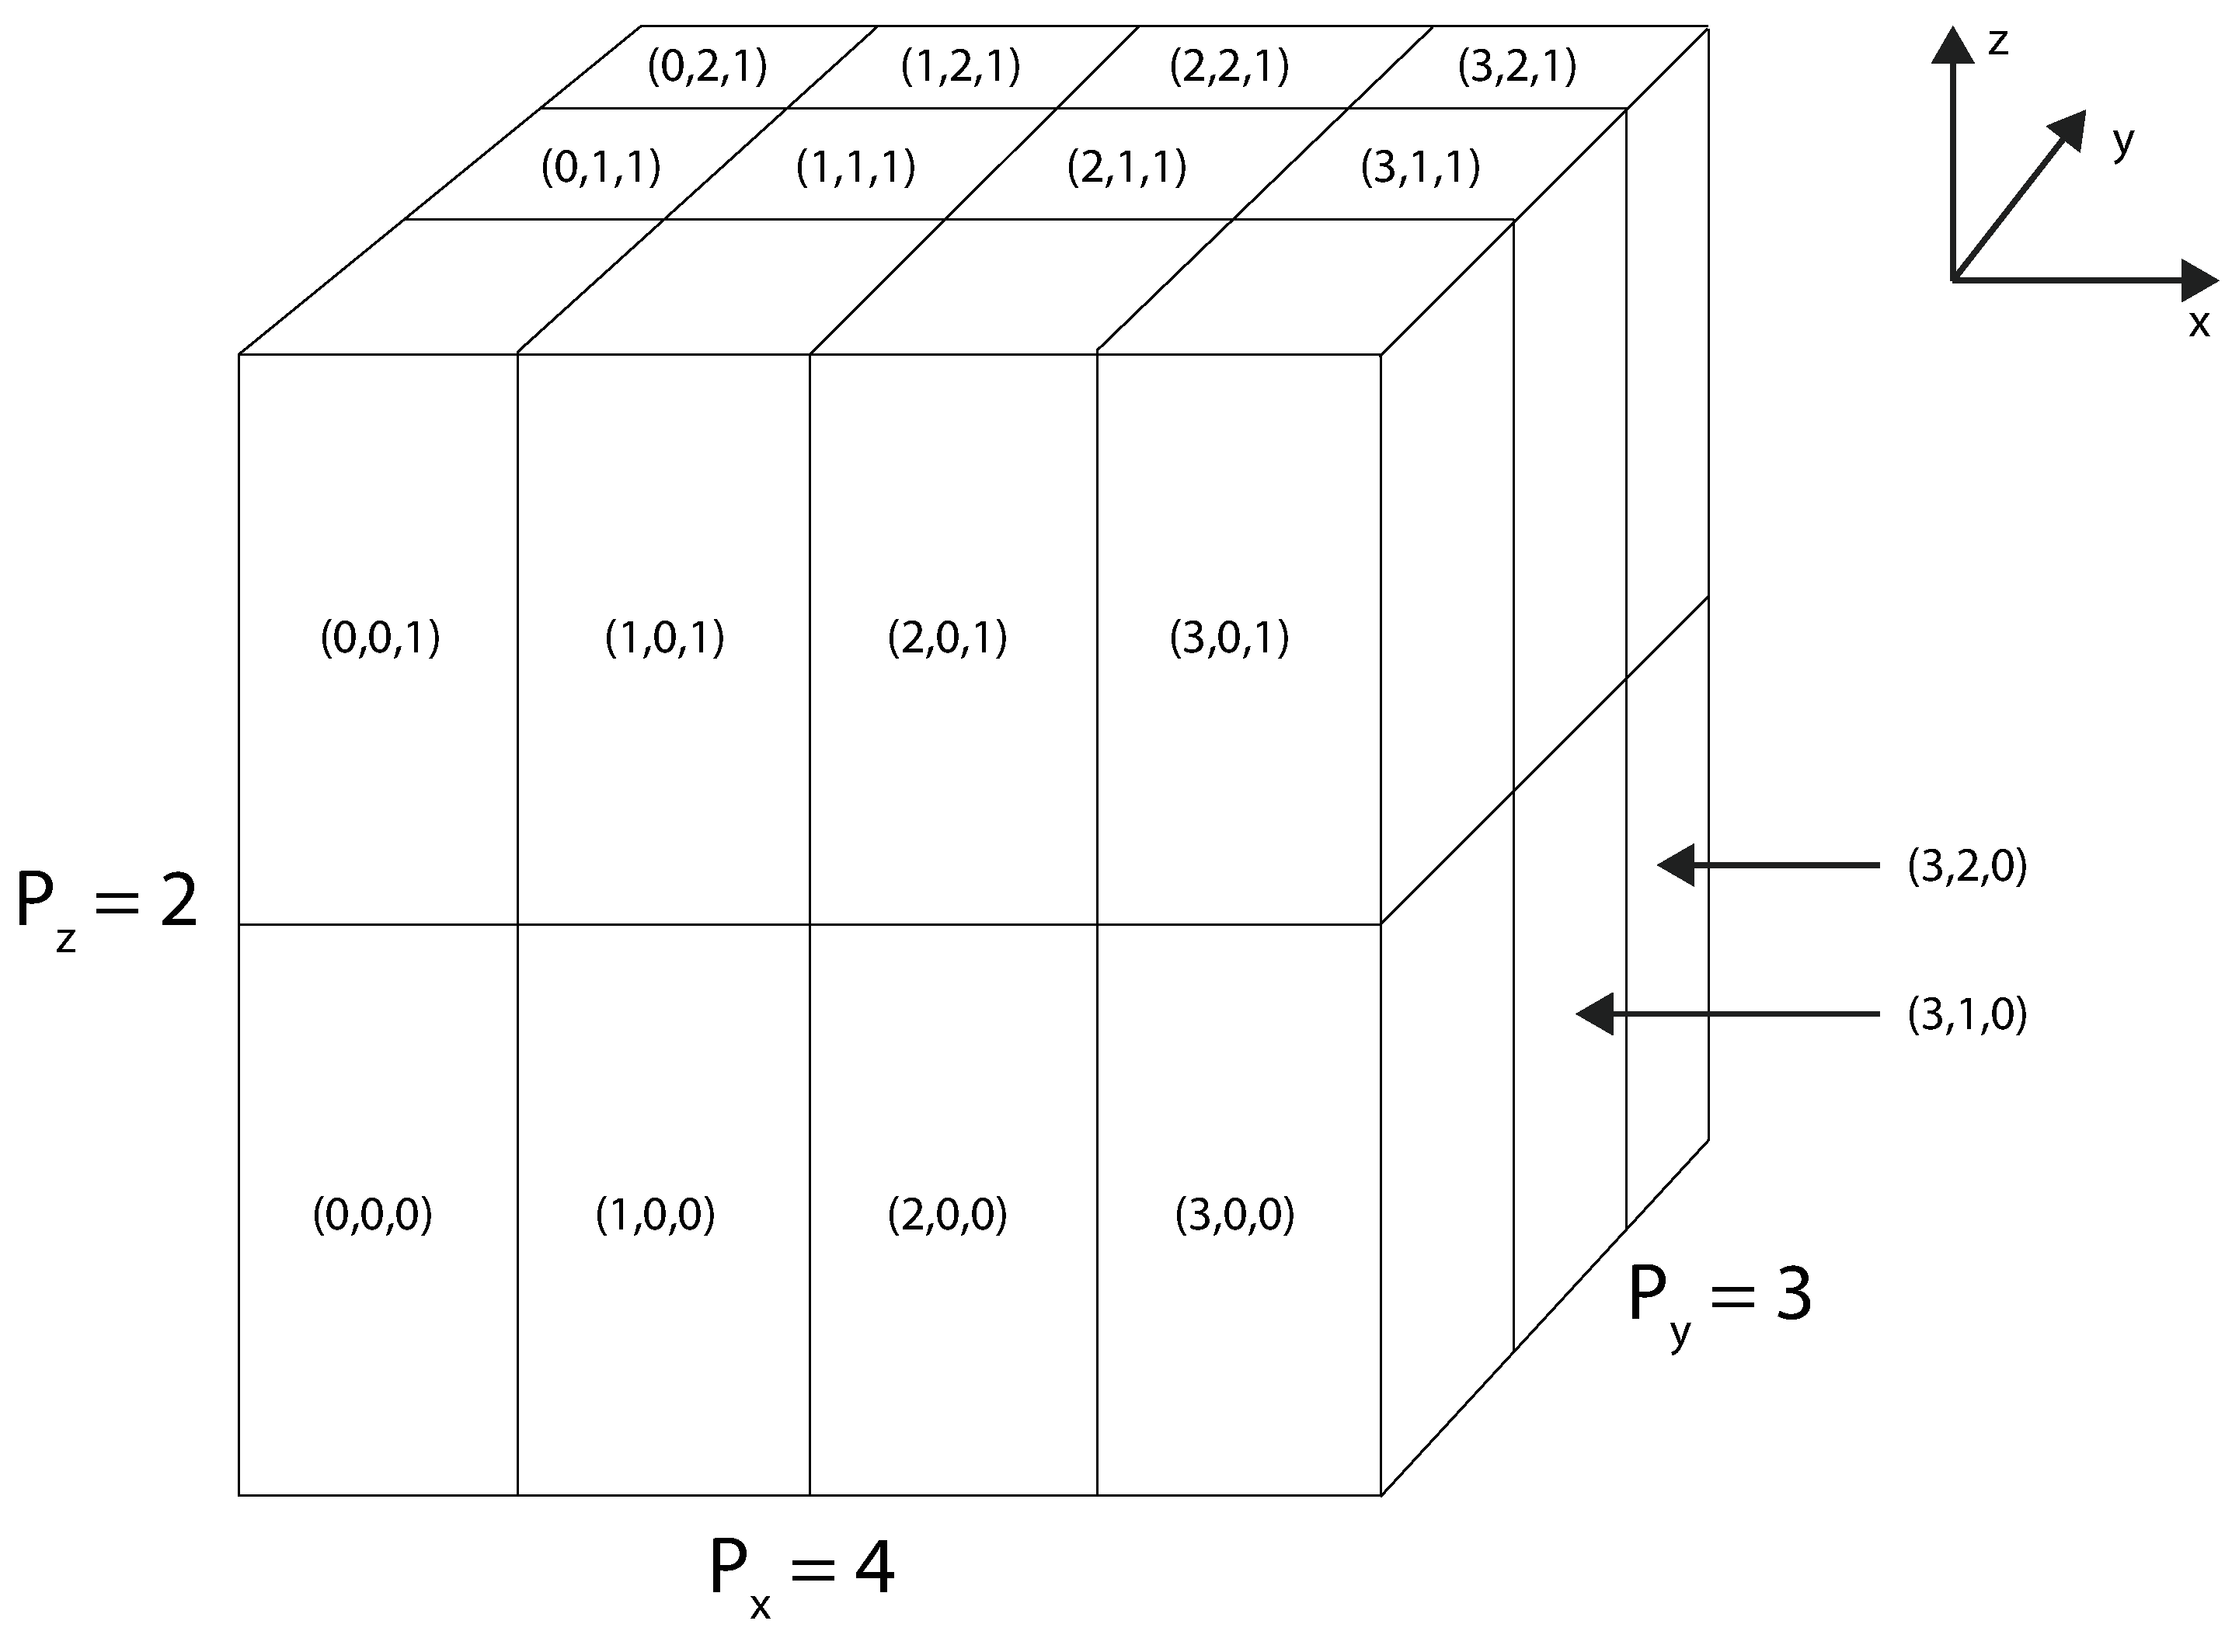
\includegraphics[width=0.7\textwidth, trim=0cm 0cm 0cm 0cm, clip]{DSMC/figures/parallelization_node_configuration.eps}
\end{center}
\caption{Processor labeling in a 3-dimensional grid. Each processor is uniquely identified through its coordinate $(p_x, p_y, p_z)$.}
\label{fig:dsmc_parallelization_2}
\end{figure}
When starting a program with MPI, each process is provided a unique identification number $p$ in the range $[0, P-1]$ for $P$ processors. This can be mapped to the 3-dimensional grid coordinates through
\begin{align}
	\nonumber
	p_x(p) &= \frac{p }{ P_yP_z}\\
	\nonumber
	p_y(p) &= \frac{p }{ P_z} \bmod P_y\\
	p_z(p) &= p \bmod P_z
\end{align}
whereas the inverted mapping is 
\begin{align}
	p(p_x, p_y, p_z) = p_xP_zP_y + p_yP_z + p_z.
\end{align}
With the processor id $p$ given, it is easy to determine which sub volume this processor should control. If the system is of size $L_i$ in the $i$'th dimension, we can find the \textit{node length} $L_i^{\text{node}} \equiv l_i = L_i/P_i$. A processor with coordinates $(p_x, p_y, p_z)$ will control all particles with coordinates in the range
\begin{align}
	\nonumber
	x&\in[p_xl_x, (p_x+1)l_x\rangle\\
	\nonumber
	y&\in[p_yl_y, (p_y+1)l_y\rangle\\
	z&\in[p_zl_z, (p_z+1)l_z\rangle.
\end{align}
Since the collision cells are independent of each other, collisions will happen in parallel where each processor loops through all of its cells colliding the particles as described in section \ref{sec:dsmc_implementation_timestep}. 
\subsection{Exchanging particles}
\label{sec:dsmc_parallelization_exchange_particles}
During a timestep, a particle can move from one processor to one of the 26 neighboring nodes (the middle node in a $3\times3\times3$ grid has a 26 neighbors). After each timestep, all processors loop through their particles to find the ones having moved out of the processor's spatial domain. This process is illustrated in listing \ref{lst:dsmc_detecting_particles_moved_out}.
\begin{lstlisting}[caption=Detecting which particles moved out of a processor's spatial domain., label=lst:dsmc_detecting_particles_moved_out]
double mpi_move() {
	for(int n=0; n<num_particles_local; n++) {
		int node_id = topology->index_from_particle_index(n);
		if(node_id != myid) {
			// Particle belongs to another node
		}
	}
}
\end{lstlisting}
In principle, there are 26 potential receiving nodes, so each node needs to be able to send information to all of them. The easiest way to implement this is to let each processor directly communicate with all of its neighbors. However, this approach requires a lot more communication time than actually needed.

If we instead send information about these particles through a 3-step process, we can reduce the number of neighboring nodes from 26 to 6. This idea is best illustrated in two dimensions, but is easily generalized to the three-dimensional case, see figure \ref{fig:parallelization_facet_technique}.
\begin{figure}[htpb]
\begin{center}
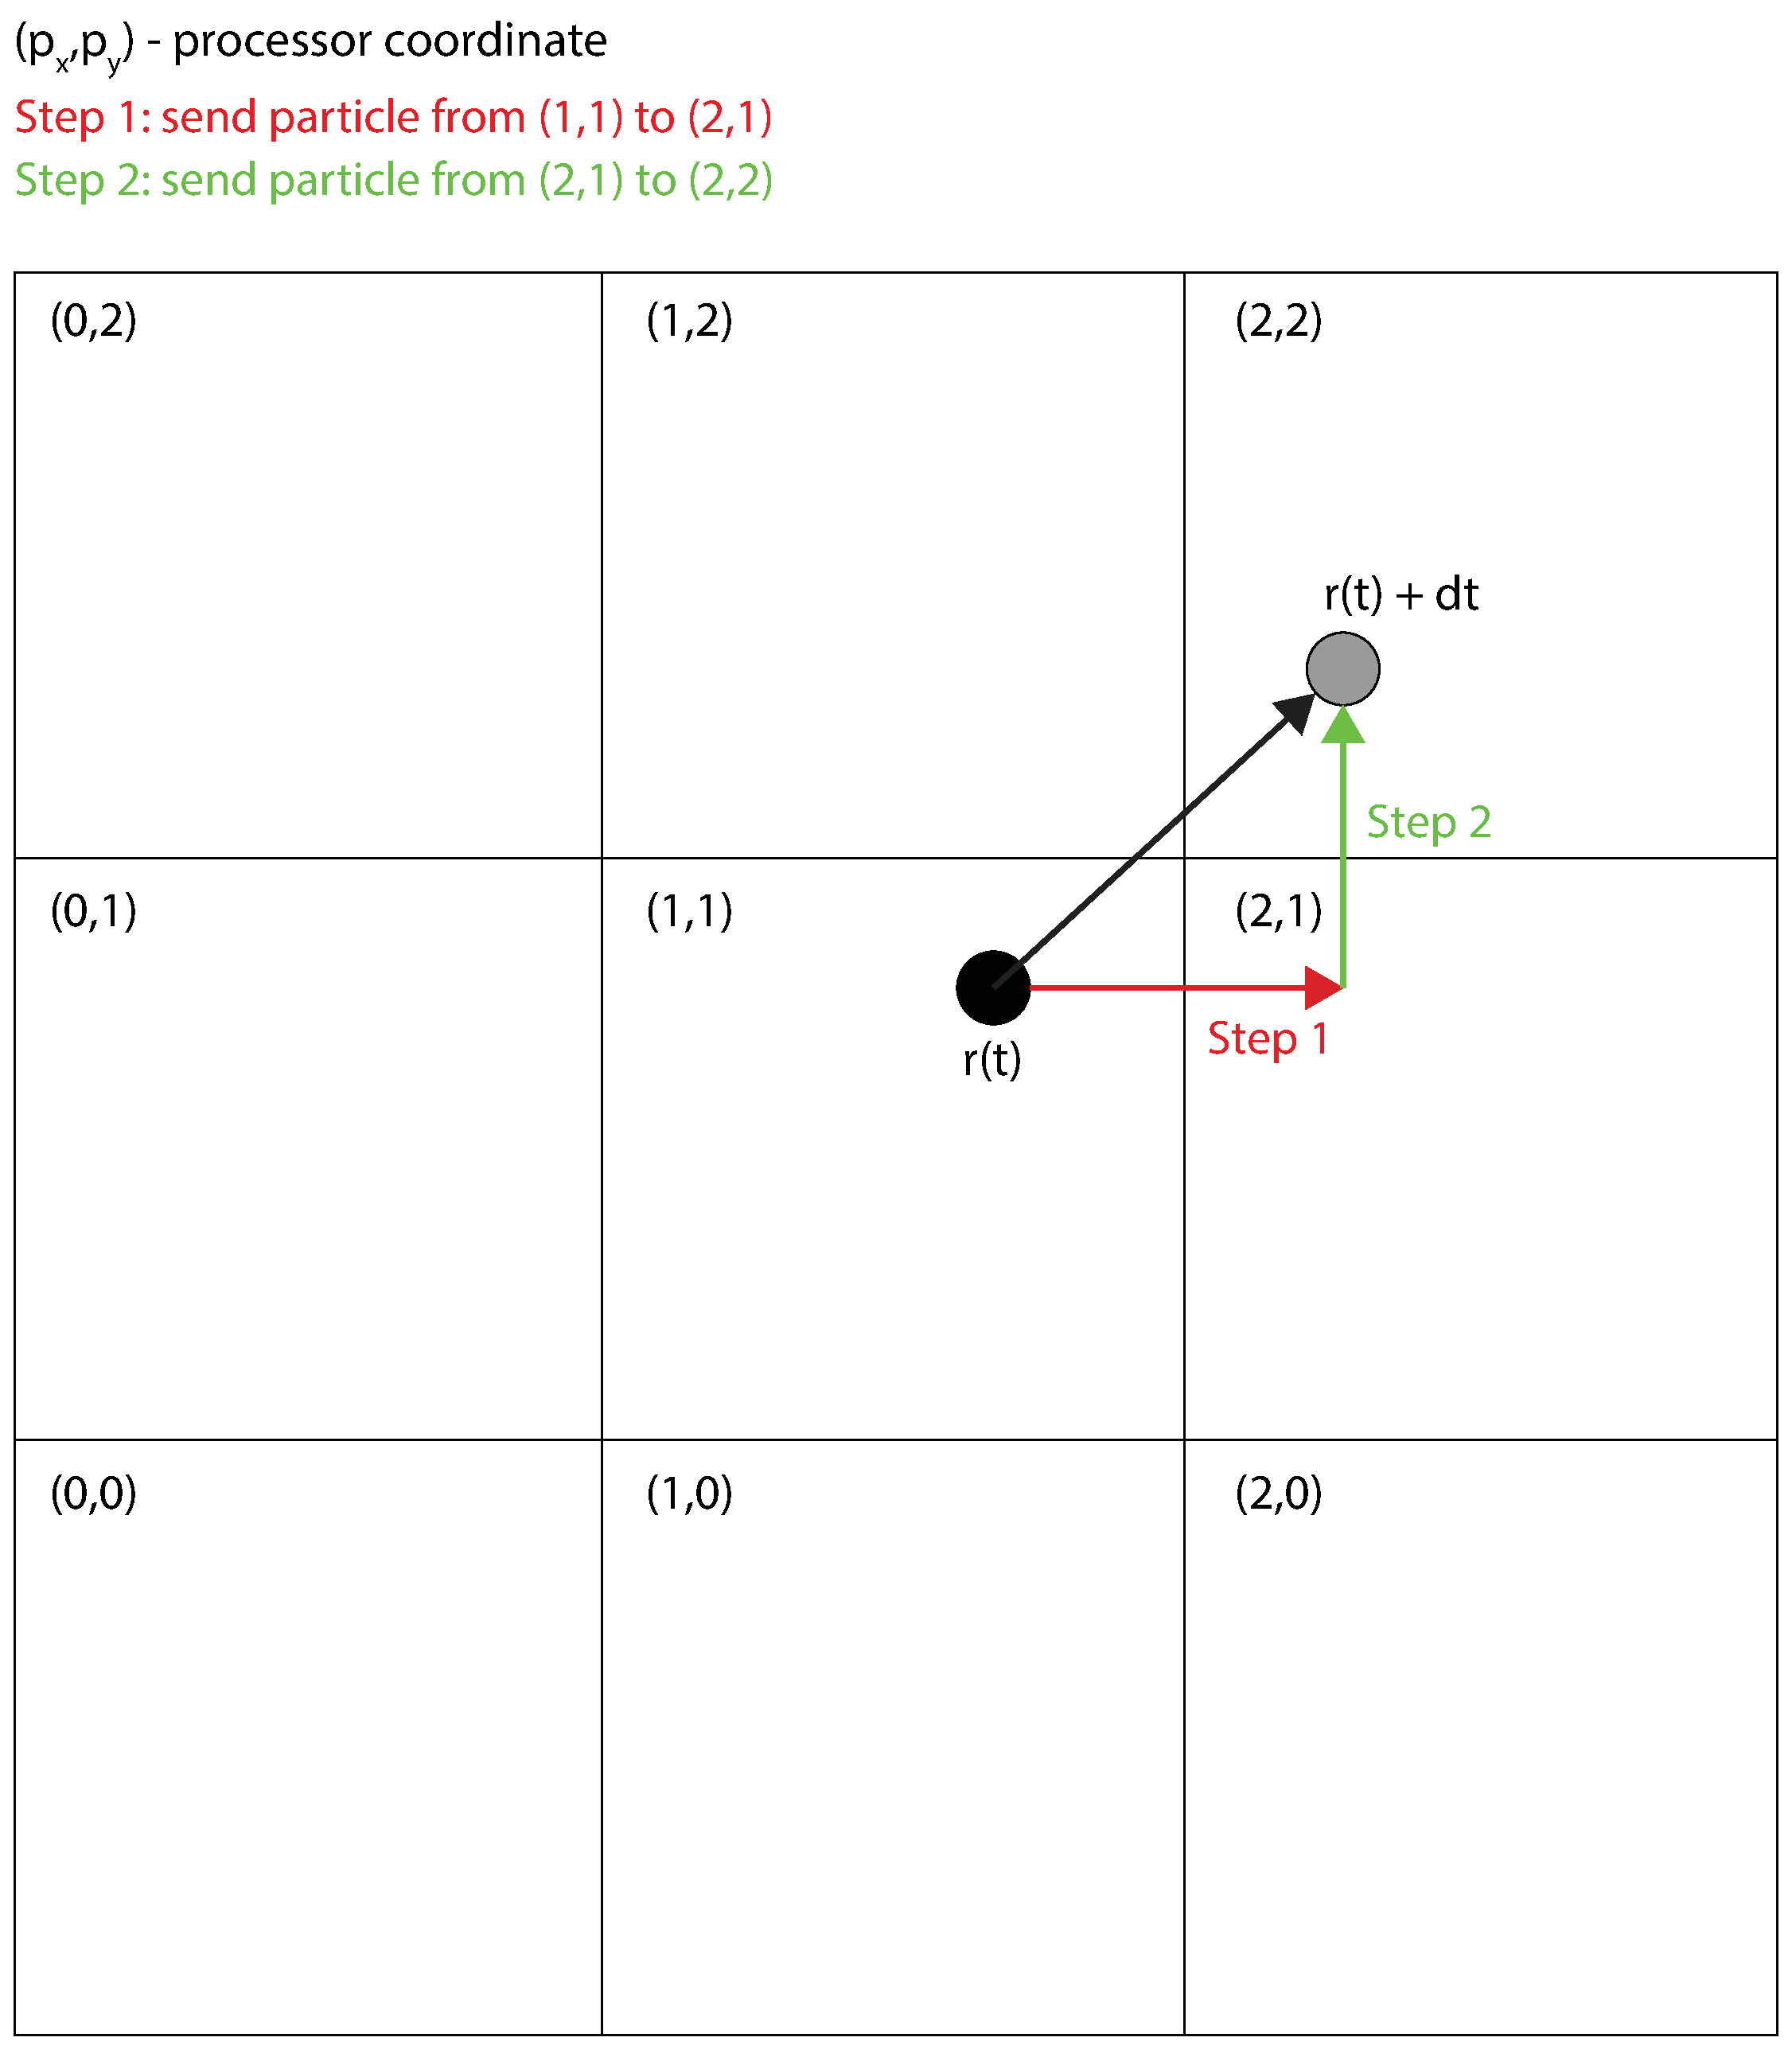
\includegraphics[width=0.7\textwidth, trim=0cm 0cm 0cm 0cm, clip]{DSMC/figures/parallelization_facet_technique.eps}
\end{center}
\caption{The middle node (1,1) has 8 neighbors it needs to communicate with. Each node only needs to communicate with its nearest neighbors (4 in two dimensions, 6 in three dimensions), because the nearest neighbors can work as intermediate information carriers. A particle that moves from processor (1,1) to (2,2) will in step 1 be sent to (2,1), then in step 2 be sent to (2,2).}
\label{fig:parallelization_facet_technique}
\end{figure}
An analysis of the parallelization is studied in subsection \ref{sec:dsmc_parallelization_performance} where we compare how well the program performance scales with increasing number of processors. 